\section{Verwendete Werkzeuge}
\label{sec:Werkzeuge}
Im Folgenden werden die Hardware und Software vorgestellt, welche die Autoren zum Erstellen dieser Arbeit und vor allem zur Entwicklung der App verwendet haben. Es wurden ausschliesslich Open-Source-Programme eingesetzt.\\
Hier benutzte Beschreibungen k�nnen von Website (offizielle Site der Software, Wikipedia...) �bernommen sein. Dieser Abschnitt dient zur Information f�r die verwendeten Werkzeuge.
\subsection{Software}
\begin{itemize}


\item \textbf{\LaTeX} \\
Diese Arbeit wurde mit {\LaTeX} geschrieben. Als Distribution und Editor wurde auf dem Mac OS Mountain Lion TexShop verwendet, auf Basis von Linux \textcolor{red}{????????????}. \\
Websites: \url{http://pages.uoregon.edu/koch/texshop/}
\end{itemize}

\subsection{Hardware}

\begin{itemize}

\item \textbf{Galaxy Nexus} \\
\index{Galaxy Nexus} \index{Jelly Bean}
Auf diesem Smartphone l�uft das brandaktuelle Andoid OS 4.1.1 (Jelly Bean).\\
\begin{tabular}[t]{|l|l|c|} \hline
\cellcolor{darkgrey} &  \cellcolor{darkgrey} & \\
\cellcolor{darkgrey} \multirow{-2}{3cm}{\textbf{Bezeichnung}} &
\cellcolor{darkgrey} \multirow{-2}{4.5cm}{\textbf{Version}} &  \\
model number & Galaxy Nexus & \\ \cline{1-2}
Android-Version & 4.1.1 (Jelly Bean) &\\ \cline{1-2}
Baseband-Version & I9250XXLF1 &\\   \cline{1-2}
Kernel-Version & 3.0.31-g6fb96c9 &\\  \cline{1-2}
Build number & JR003C.I9250XWLH2 & \\  \cline{1-2}
Screen Resolution & 1280 x 720 pixel & \\ \cline{1-2}
diagonal & 4.65 inch & \multirow{-8}{5.0cm}{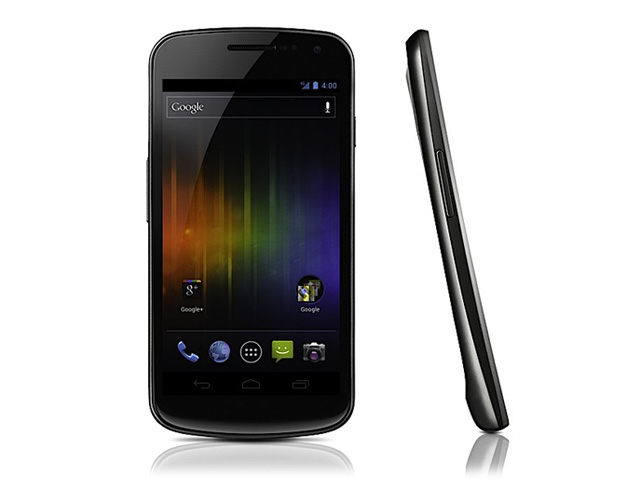
\includegraphics[width=5.0cm]{galaxynexus.png} }\\  \hline 
\end{tabular}\\


\item \textbf{HTC Desire HD A9191} \\
\index{HTC Desire} \index{Froyo}
\begin{tabular}[t]{|l|l|c|} \hline
\cellcolor{darkgrey} &  \cellcolor{darkgrey} & \\
\cellcolor{darkgrey} \multirow{-2}{3cm}{\textbf{Bezeichnung}} &
\cellcolor{darkgrey} \multirow{-2}{4.5cm}{\textbf{Version}} &  \\
model number & HTC Desire HD A9191 & \\ \cline{1-2}
Android-Version & 2.3.5 (Gingerbread) & \\ \cline{1-2}
Baseband-Version &  \textcolor{red}{$12.65.60.29U\_26.14.04.28\_M$} & \\ \cline{1-2}
Kernel-Version & 2.6.35.10-g931a37e & \\ \cline{1-2}
Build number &   3.13.163.3 CL208029 & \\ \cline{1-2}
Screen Resolution & $800 � 480$ pixel & \\ \cline{1-2}
diagonal & 4.3 inch &  \multirow{-8}{5.0cm}{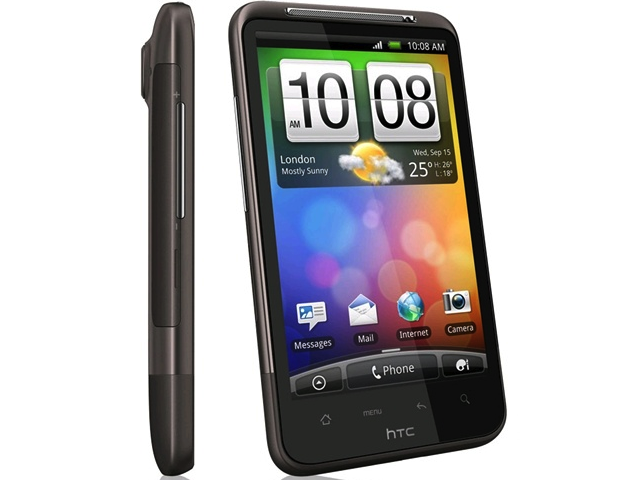
\includegraphics[width=5.0cm]{HTC_Desire_HD_A9191.png} }\\  \hline 
\end{tabular}\\
\end{itemize}



